%%%%%%%%%%%%%%%%%%%%%%%%%%%%%%%%%%%%%%%%%%%%%%%%%%%%%%%%%%%%%%%%%%%%%%%%%%%%%%%%

% IEEEconf.cls file must exist in the same directory as the TeX file you want to compile
\documentclass[letterpaper, 10 pt, conference]{IEEEconf}

\usepackage{hyperref}
\hypersetup{
    colorlinks=true,
    linkcolor=blue,
    filecolor=magenta,      
    urlcolor=blue,
    citecolor=black
    }
    
% Image/graphics support
\usepackage{graphicx}
\graphicspath{ {./images/} }

\title{\LARGE \bf
MACINTOSH COMPUTER HISTORY\\
\large The 1984 Macintosh
}

\author{Group Number Seven\\
\small Dominic Martinez\\
\small Keilahna McFall\\
\small Sarah Crotzer\\
}

% Formatting for lists
\usepackage{enumitem}

% Formatting for media
\usepackage{float}
\restylefloat{table}
\restylefloat{figure}

\begin{document}


\maketitle
\thispagestyle{empty}
\pagestyle{empty}

\begin{figure}[h!]
\centering
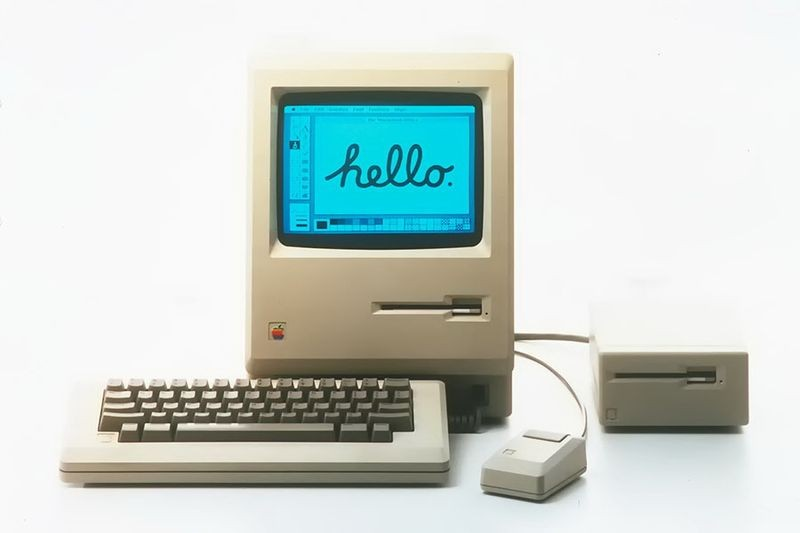
\includegraphics[width=0.45\textwidth]{hw3/images/applemacintosh.jpg}
\caption{The first Apple Macintosh \cite{HelloMacPic}}
\label{fig:example}
\end{figure}

%%%%%%%%%%%%%%%%%%%%%%%%%%%%%%%%%%%%%%%%%%%%%%%%%%%%%%%%%%%%%%%%%%%%%%%%%%%%%%%%

\section{INTRODUCTION}

Looking back on the history of computers, the 1984 Apple Macintosh played a major part in building technology into what it is today. It introduced new hardware and concepts in the architecture in computers, and began a new era of computer programs and software. The Macintosh also made a mark on the market from the day it was released, January 24, 1984, for a price of  \$2,500 \cite{HelloMacPic}. This computer helped to revolutionise technology.

%%%%%%%%%%%%%%%%%%%%%%%%%%%%%%%%%%%%%%%%%%%%%%%%%%%%%%%%%%%%%%%%%%%%%%%%%%%%%%%%

\section{TIME PERIOD (1980s)}

The 1980s were a time of revolution for technology, with the release of PCs and the idea of having this brand new technology at home. It seemed that new computers or technologies were being introduced left and right. Some of the major companies of the time that were constantly competing were IBM and Apple, the competition starting in 1983 when IBM released a new PC right after the flop of Apple's Lisa \cite{MacHistory}. 

However, 1984 was the turning point of all this, and what really changed the tech industry and the public's perception of them. At the time, there were speculations that the world was going to turn into the dystopian world depicted in George Orwell's novel \textit{1984}. Apple built off this concept when creating the Super Bowl ad to announce the release of the Macintosh \cite{HelloMacPic}.

\begin{figure}[h!]
\centering
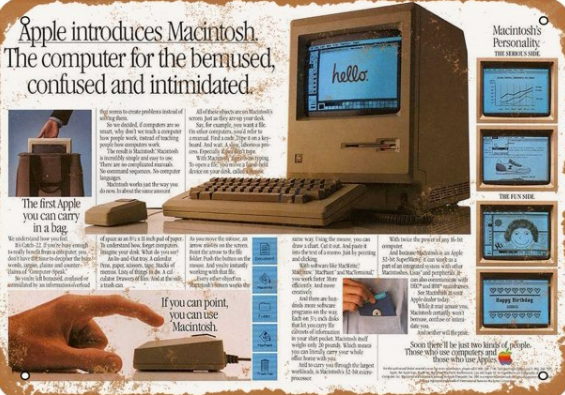
\includegraphics[width=0.45\textwidth]{hw3/images/applemacintoshad.png}
\caption{Apple Macintosh Ad \cite{MacAd}}
\label{fig:example}
\end{figure}

The Macintosh was the turning table for this revolution of technology in the 80's, and helped to change the point of view of the public and their scepticism on the new technology.

%%%%%%%%%%%%%%%%%%%%%%%%%%%%%%%%%%%%%%%%%%%%%%%%%%%%%%%%%%%%%%%%%%%%%%%%%%%%%%%%

\section{COMPUTER HARDWARE}

The hardware that made up the 1984 Macintosh included 64 Kb of ROM and 128 KB of RAM, the Motorola 68000 microprocessor with a speed of 8MHz, and was capable of supporting a 9-inch, 512×342 pixel monochrome display, \cite{MacHardware}.

Although there were no memory slots, the RAM was expandable by the soldering of sixteen chip sockets to accept 256 Kb RAM chips in place of the factory-installed chips.  The Mac also lacked an internal hard drive and did not have a fan, causing many of its components to fail. Due to the lack of a fan, the Mac was soon after nicknamed "The Beige Toaster" \cite{BeigeToster}.

The Macintosh also incorporated a mouse and graphical user interface, which were unusual among other personal computers.

\section{COMPUTER SOFTWARE}

The Macintosh ran on the Classic Mac Operating System, which was named Mac System 1.  Although it was criticized for a lack of "modern technologies" compared to it's competitors, the Mac OS is also credited for the popularization of the graphical user interface concept \cite{enwiki:1046320952}.  Features included the Finder, menu bar and various desktop accessories and applications.

\begin{figure}[h!]
\centering
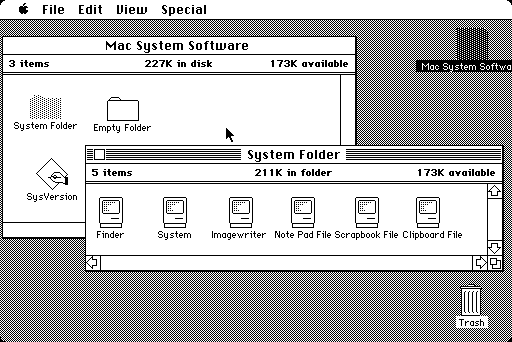
\includegraphics[width=0.45\textwidth]{hw3/images/AppleSoftware.png}
\caption{System Software and Finder \cite{SoftwarePic}}
\label{fig:example}
\end{figure}

Application software included on the Macintosh included MacPaint and MacWrite.  MacPaint was a graphics editor that could generate images that could be used in other applications.  MacWrite was a WYSIWYG word processor, and it set the precedent for GUI-based word processors.

Only one application could run at a time, and because the computer was centered around GUI, the command-driven applications had to be re-designed and re-programmed, which was a time intensive process that resulted in an initial lack of software \cite{MacHardware}.

\section{CONCLUSION}

I was surprised to learn that the Apple Macintosh was the first to include a lot of unusual components such as mice and a graphical user interface with a pixel display.  I thought that these now commonplace components would have been integrated in earlier personal computers.  It was also surprising to learn that the Macintosh had various issues upon it's release, such as an initial lack of software, no fan or internal hard drive, and very limited memory.

Even in spite of the complications with hardware, software and even advertisements and pricing, the Macintosh paved the way for Graphical User Interface based personal computers and ultimately led to the widespread success of Apple.

%\section*{REFERENCES} looks kinda wierd ngl

\bibliographystyle{acm}
\bibliography{sources}

\end{document}

